%
% ldmx_cdr.tex
% date: July 09, 2016
%
% Set the document type and the font size
\documentclass[11pt]{article}

%%%%%%%%%%%%%%%%
%   Packages   %
%%%%%%%%%%%%%%%%
\usepackage{jheppub}	
\usepackage{url}
\usepackage{graphicx}
\usepackage{amssymb}
\usepackage{bm}
\usepackage{color}
\usepackage{mathrsfs}
\usepackage{amsmath}
\usepackage{amsfonts}
%\usepackage{hepunits}
\usepackage{color}
\usepackage{tikz}
\usepackage{slashed}
\usepackage{cancel}
\usepackage{hyperref}
\usepackage[utf8]{inputenc}											
\usepackage{slashed}
\usetikzlibrary{arrows}
\usetikzlibrary{shapes}
\usetikzlibrary{trees}
\usetikzlibrary{matrix}
\usetikzlibrary{arrows} 			
\providecommand{\draft}[1]{{\color{blue}#1}}
%%%%%%%%%%%%%%%%%%%%%%%%%%%
%%%% Gordan's packages for goals section %%%%
%%%%%%%%%%%%%%%%%%%%%%%%%%%
%\usepackage{amssymb,graphicx,cancel}
%\usepackage[margin=2cm]{geometry}
\usepackage{graphicx,epsfig,psfrag,bm,amssymb}
\usepackage{dcolumn}
\usepackage{bm}
\usepackage{color}
\usepackage{mathrsfs,amsfonts,hepunits,color}
\usepackage[utf8]{inputenc}
\usepackage{epsfig,latexsym,cancel,amssymb,amsmath,mathrsfs}
\usepackage{graphicx}
\usepackage{epstopdf}
\usepackage{mciteplus}
\usepackage{latexsym}
\usepackage{amsthm}
\usepackage{amsmath}
\usepackage{amssymb}
\usepackage{hepunits}
\usepackage{hyperref}
\usepackage{bbm}
\usepackage{bm}
\usepackage{xfrac}
\usepackage{color}
\usepackage{colordvi}
\usepackage{comment}
\usepackage{dcolumn}
\usepackage{times,latexsym,graphicx,wrapfig}
\usepackage{epsfig,lineno,bm}
\usepackage{subfigure}
\usepackage{slashed}
\newcommand{\be}{\begin{eqnarray}}
\newcommand{\ee}{\end{eqnarray}}
\newcommand{\Gev}{\,\,\mathrm{GeV}}
\newcommand{\SUWeak}{\mathrm{SU}(2)_{\rm W}}
\newcommand{\Lag}{\mathcal{L}}
\newcommand{\Lagtree}{\mathcal{L}_{\rm tree}}
\newcommand{\benum}{\begin{enumerate}}
\newcommand{\eenum}{\end{enumerate}}
\newcommand{\bi}{\begin{itemize}}
\newcommand{\ei}{\end{itemize}}
\newcommand{\met}{\slashed{E_T}}
\newcommand{\ap}{{A^\prime}}
%%%%%%%%%%%%%%%%%%%%%%%
%%%%%%%%%%%%%%%%%%%%%%%
\begin{document}

%%%%%%%%%%%%%%%%
% Front Matter %
%%%%%%%%%%%%%%%%

% 
% Front matter should be moved to its own page
%
\title{Light Dark Matter eXperiment (LDMX): \\ Letter of Intent}

\author[a]{an author}
\affiliation[a]{an institution}

\abstract{The LDMX experiment proposes a high-statistics search for low-mass dark matter at the DASEL beamline using the missing momentum technique, scattering incoming electrons in a tungsten target to produce dark matter via ``dark bremsstrahlung''. This clear signature is established by individually tagging incoming beam-energy electrons and unambiguously associating them with low energy, moderate transverse-momentum recoils and establishing the absence of a forward-going photon. The primary backgrounds are traditional bremsstrahlung processes with photo-nuclear reactions occurring in the target or forward calorimeter. Therefore, the experiment requires a high-speed, granular calorimeter with MIP sensitivity to identify rare photo nuclear reactions, in addition to low mass tracking that provides high-purity tagging for incoming electrons and clean, efficient reconstruction of recoils. The LDMX concept proposes to meet these challenges by leveraging technology under development for the HL-LHC and experience from the HPS experiment.}

\maketitle

%%%%%%%%%%%%%%%%%%%%%%%%%%%%%%%%%%%%%%
%   Overview and Executive Summary   %
%%%%%%%%%%%%%%%%%%%%%%%%%%%%%%%%%%%%%%
\section{Overview and Executive Summary}


%%%%%%%%%%%%%%%%%%%%%
%   Science Goals   %
%%%%%%%%%%%%%%%%%%%%%
\section{Science Goals (Editors: Philip Schuster, Gordan Krnjaic)}

\subsection{Testing Thermal Dark Matter}

The overwhelming evidence for the existence of dark matter (DM) arises from multiple independent sources. 
 Observations of galactic rotation curves, the power spectrum of the Cosmic Microwave Background (CMB), 
the cosmological matter power spectrum, light element yields from Big Bang Nucleosynthesis (BBN), gravitational
lensing, and galaxy cluster collisions all require roughly 85\% of the matter in our universe to be cold and non-baryonic. 
Together, these data constitute smoking gun evidence  of physics beyond the Standard Model (SM), which contains
no viable DM candidate -- for a review see \cite{Bertone:2004pz}.

However, despite this impressive body of evidence, the particle nature of DM remains completely unknown; all indications of 
its existence derive ultimately from its gravitational influence on visible matter in different contexts. 
Without making any further assumptions about these hypothetical interactions or DM's cosmological history,
 its viable mass range is wildly unconstrained: $10^{-22} $ eV -- $10 M_{\odot}$.  If DM is lighter than $\sim 10^{-22}$ eV, 
 its Compton wavelength does not fit inside the smallest known DM dominated objects \cite{Navarro:1995iw} and if it's heavier than $\sim 10 M_{\odot}$ 
 it would have distorted the CMB power spectrum at early times \cite{Bird:2016dcv}. Given such an enormous range of viable masses, a realistic DM discovery effort requires a well motivated organizing principle to manageably and systematically test this vast space of possibilities without being narrowly tailored
 to specific models.

\subsubsection{Thermal Origin}
A compelling, well motivated organizing principle for the DM search effort is the hypothesis that DM
is produced through its interactions with the SM in thermal equilibrium during the early universe. This criterion
selects a broad class of popular DM models (including Supersymmetry) and is defined by the requirement that the DM-SM 
interaction rate exceed the Hubble expansion rate at early times.  
Once achieved, thermal equilibrium offers some generically attractive features that do not depend sensitively
on particular model details:
\begin{itemize}
\item {\bf Generically Realized:} Equilibrium is hard to avoid even with tiny coupling constants  between 
dark and visible matter; thus, most {\it discoverable} models of DM with non-gravitational interactions fall into this category. 
Alternative mechanisms (e.g. axions produced via misalignment \cite{Visinelli:2009zm} or feebly coupled DM produced via freeze in \cite{Hall:2009bx}) require such small couplings
that comprehensive experimental probes are prohibitively difficult in most regions of their parameter space -- see \cite{Essig:2013lka}.
\item {\bf Minimum Annihilation Rate:}  Equilibrium at temperature $T$ populates the DM with a  thermal number density $n_{\rm DM} \propto T^3$, which is many orders of magnitude larger than the observed abundance. Thus, viable thermal DM must be depleted with an annihilation cross section $\sigma v \ge 3\times10^{-26}$ cm$^3$/s via
the process of thermal ``freeze out." This inequality must be saturated (=) if DM is particle/antiparticle symmetric and exceeded ($>$)  if there is an additional primordial DM asymmetry which contributes to the total abundance in addition to the freeze-out component.

\item {\bf Narrower Mass Window: }The viable DM mass range becomes much narrower -- see Fig. \ref{fig:schematic}.
Thermal DM below $\lesssim$ 10 keV erases small scale structure in conflict with observation; 
thermal DM above $\gtrsim$ 10 TeV requires nonperturbative and/or non-unitary couplings to realize
a sufficiently large annihilation rate. 
\end{itemize}

\subsubsection{``WIMP" Dark Matter}
If thermal DM is realized in the upper half of the thermal mass window $\sim$ GeV - 10 TeV, it can be a Weakly Interacting Massive Particle (WIMP) charged under the 
familiar electroweak force and achieve the observed
relic abundance by annihilating through via SM gauge interactions.  This class of models exploits the numerical
 coincidence between electroweak-sized cross sections and the requisite annihilation cross section for thermal freeze out $\sigma \sim \alpha^2 /m_Z^2  \to \sigma v \sim 3 \times 10^{-26}$ cm$^3$/s (see \cite{Kolb:1990vq} for a pedagogical treatment). This so-called ``WIMP miracle" also naturally arises in popular extensions of the SM that address the electroweak hierarchy problem 
(e.g. Supersymmetry and extra dimensions) and may even be realized with fifth forces beyond the SM so long as the appropriate coupling-to-mass
ratio is of electroweak size, but the latter possibility is not obligatory for masses in the WIMP range.  

\begin{figure}[t!]
\center
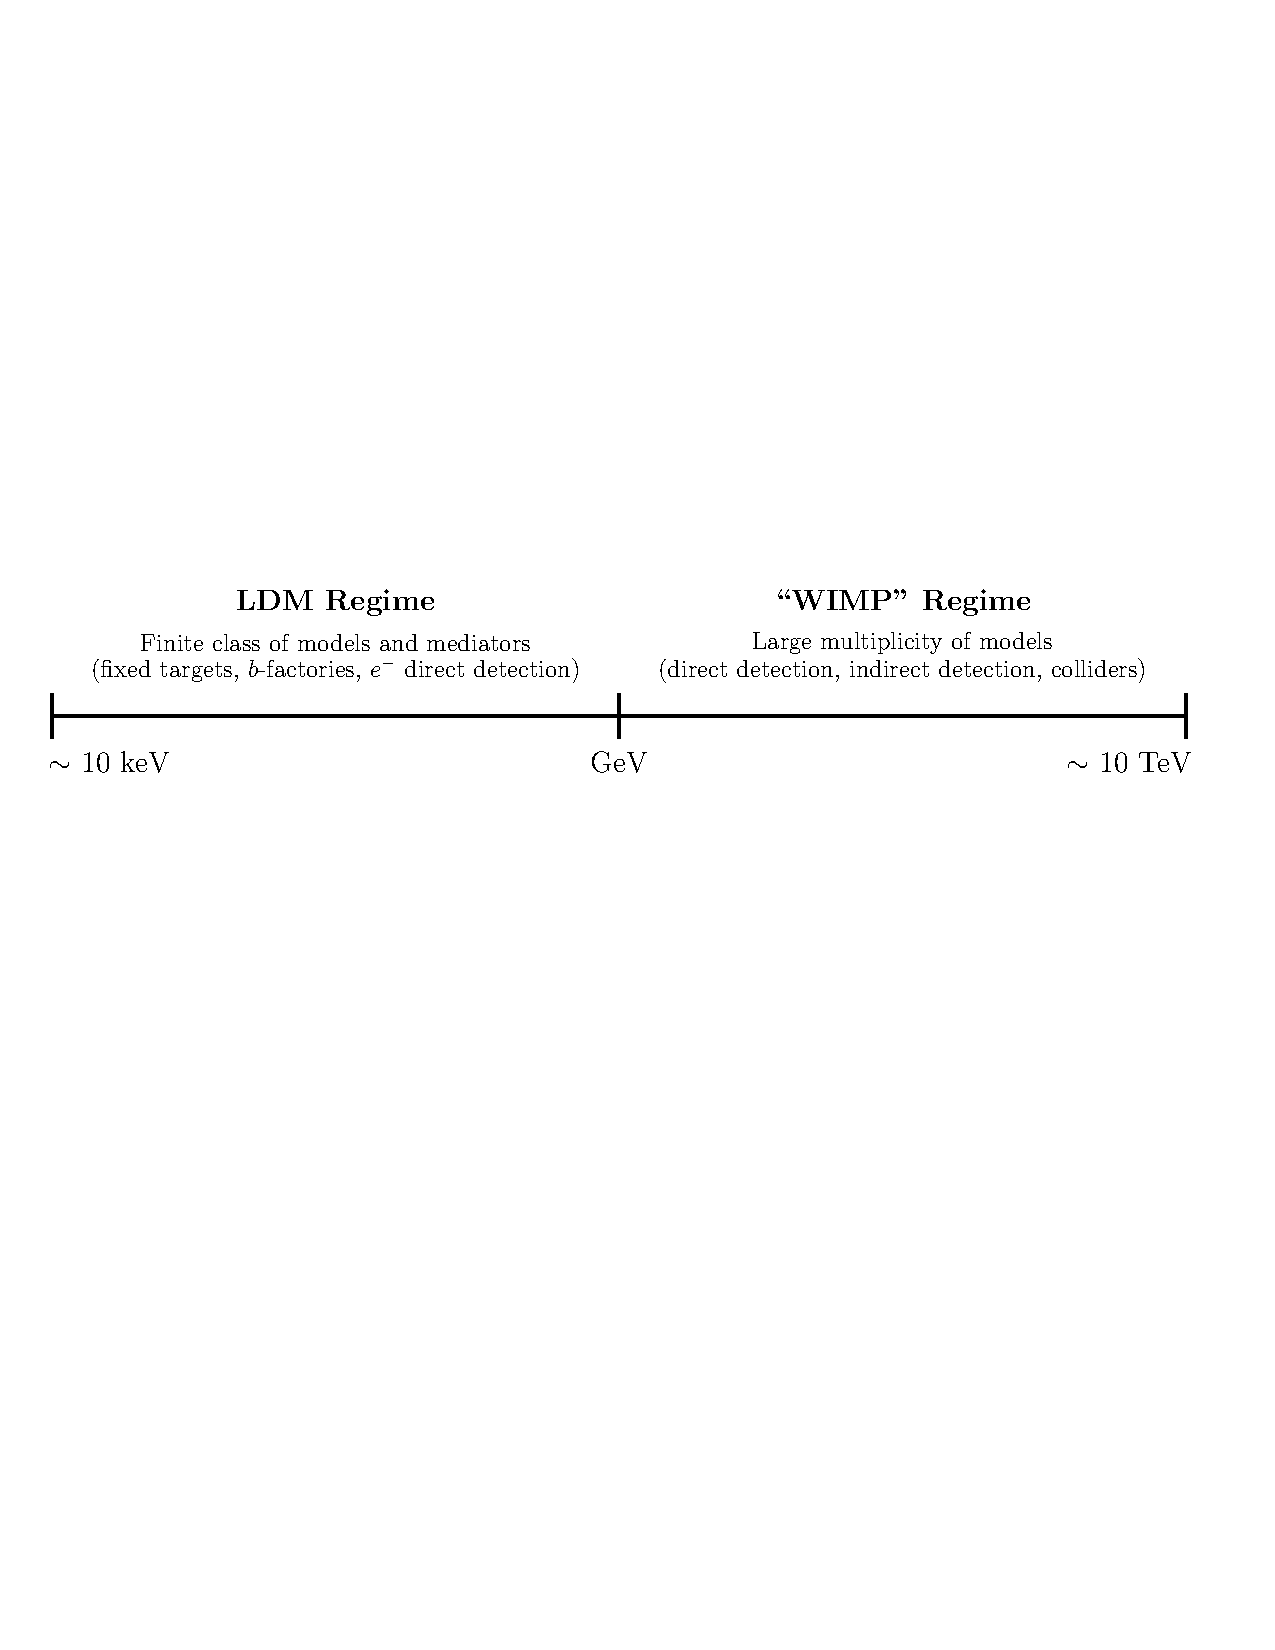
\includegraphics[width=15cm]{sections/goals/schematic.pdf}
\caption{The allowed mass range over which DM can thermalize with the SM in the early universe and yield the observed relic abundance via 
annihilation. For masses below $\lesssim 10$ keV, DM is too hot to form the observed structure of the universe on large scales  \cite{Viel:2013apy} and for masses above $\gtrsim 10$ TeV, a perturbative annihilation rate cannot achieve the correct relic abundance in simple models \cite{Griest:1989wds}. }
\label{fig:schematic}
\end{figure}

The discovery techniques available for WIMP and WIMP-like DM are well known and firmly established the experimental community:
\begin{itemize}
\item {\bf Direct Detection:} Terrestrial searches for non relativistic WIMP-nucleon scattering in a shielded underground detector \cite{Undagoitia:2015gya}. This technique 
is powerful for DM masses near $\sim$ 10 GeV - 10 TeV, but loses sensitivity near the GeV where typical nuclear recoils are $\lesssim$ keV,
below detection sensitivity thresholds. The sensitivity of this approach depends critically on the presently unknown DM velocity distribution in the 
terrestrial neighborhood and is therefore subject to potentially large systematic uncertainties. 

\item {\bf Indirect Detection:} Typically space based searches of DM annihilation in regions of high DM density (galactic center, dwarf galaxies etc.) \cite{Conrad:2014tla}.
This technique is approaching sensitivity to thermal DM annihilation rates for a variety of scenarios, but poorly constrains DM below the 
few-GeV scale. As with direct detection, the signal strength for indirect detection depends on an unknown DM phase space profile in regions of high density, 
so the systematic uncertainties of this approach may also be very large. 

\item {\bf Collider Production} Laboratory based searches for DM produced in association with visible final states in SM particle collisions \cite{Askew:2014kqa}. This technique
is powerful and not limited by halo uncertainties or the limitations of non-relativistic scattering off DM particles in the Earth's neighborhood. However, 
for DM below the GeV scale, the transverse missing energy in a typical production evennt is too low to impart sufficient recoil $P_T$ to the other
visible object(s) in the final state, so sensitivities remain weak for the lower half of the thermal mass window \cite{Izaguirre:2015yja}. 

\end{itemize}

\subsubsection{Light Dark Matter (LDM)}

Although the thermal freeze-out production mechanism can apply equally well to light DM (LDM) in the keV-GeV range, 
achieving the observed annihilation rate is no longer possible with SM forces. Annihilation to SM particles via virtual electroweak gauge boson exchange
scales as $\sigma v \sim \alpha^2 m_{\rm DM}^2/m_Z^4 \ll 3\times 10^{-26} $ cm$^3$/s, which is insufficient for freeze out if $m_{\rm DM} \ll m_{Z}$. Thus,
for light thermal DM to be viable:
\begin{itemize}
\item {\bf Light New Forces:} There have to be comparably light force carriers with to mediate an efficient  annihilation rate 
for thermal freeze out. 
\item {\bf Portals: } Both the DM and the mediator must be singlets under the full SM gauge group; otherwise 
 would have been produced in Z-pole measurements at LEP. Thus, in order for the DM to annihilate away its abundance, the mediator particle 
 must have a {\it renormalizable}\footnote{If the operator were not renormalizable, 
 there would have to be additional, sub-electroweak states integrated out to generate 
 such an interaction since electroweak sized suppression scales in higher dimension operators would reintroduce 
 the overproduction problem. However, the states that UV complete such an interaction would be 
 electroweak charged and ruled out by LEP searches for light, electroweak charged matter. } coupling to SM particles through a mass-dimension $< 4$ singlet ``portal" operator built out of SM fields.
\end{itemize}
The second bullet point sharply constrains the options for LDM mediator particles since the only renormalizable SM operators that
satisfy this requirement are 
\be
\hat {\cal O}_{\rm portal}   =  H^\dagger H  ~~,~~   H L ~~~, ~~~ B_{\mu\nu} ~~,~~
\ee
and are known respectively as the Higgs, lepton, and vector portals (for a discussion, see \cite{Pospelov:2008zw}). Here $H$ is the SM Higgs doublet, $L$ is the SM lepton doublet, and 
$B_{\mu \nu } = \partial_\mu B_\nu - \partial_\nu B_\mu$ is the $U(1)_Y$ hypercharge field strength tensor, which is independently gauge invariant. 
Each portal corresponds to a different choice of mediator spin -- only a scalar mediator can couple to the $H^\dagger H$ bilinear, only a fermionic mediator can couple to 
the lepton portal operator $LH$, and only a spin-1 mediator can couple to the $B_{\mu \nu}$ vector portal.
However, for the most predictive model variations, the scalar mediator is strongly disfavored by a variety of experimental constraints \cite{Krnjaic:2015mbs} 
and the lepton portal interaction is generically proportional to factors of neutrino masses $m_\nu \lesssim 0.1$ eV, so it is difficult to sustain 
thermal contact between DM and SM sectors. Thus, for the rest of this discussion, we will emphasize the vector portal as the representative mediator1
of LDM interactions. 

\begin{figure}[t!]
\center
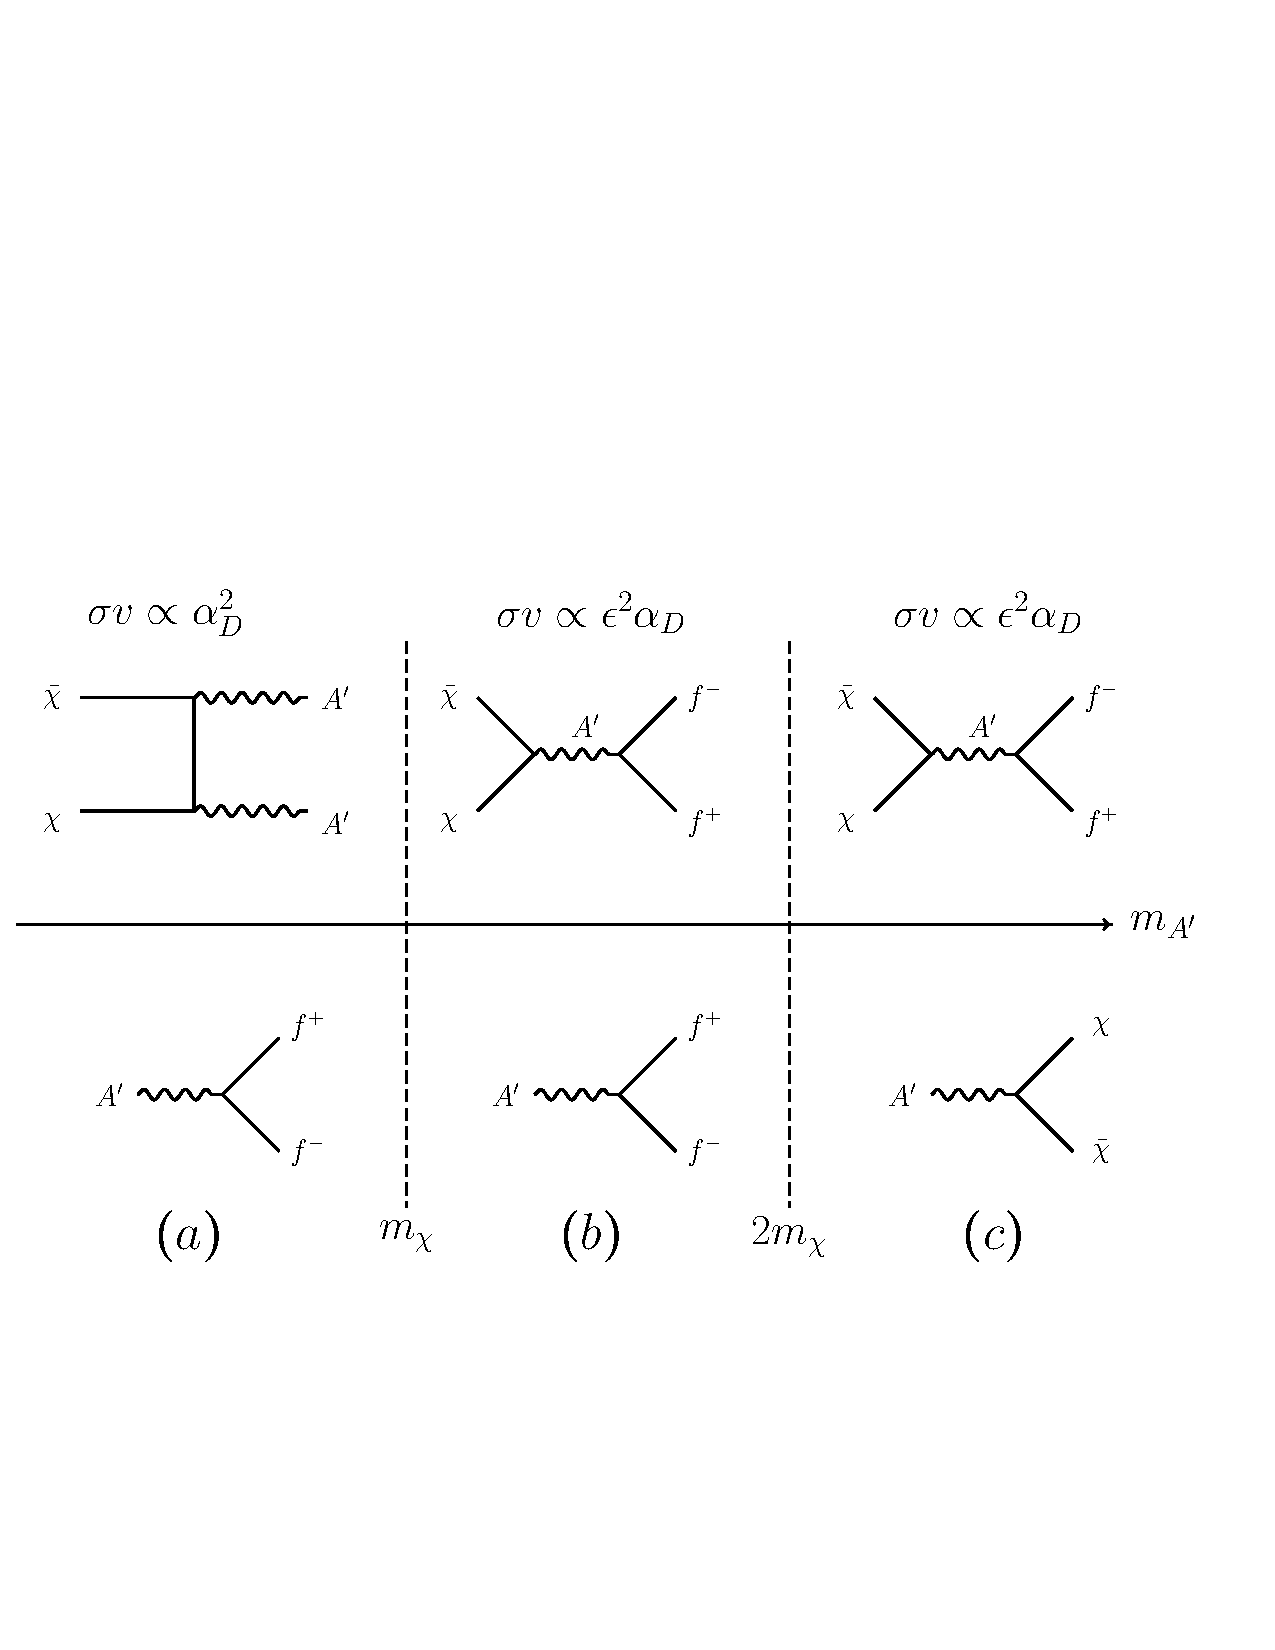
\includegraphics[width=15cm]{sections/goals/breakdown.pdf}
\caption{ Schematic representation of the different DM annihilation modes (top row) and $A'$ decay modes for $m_\chi/m_{A^\prime}$ ratios. 
a) Secluded annihilation scenario with  a visibly decaying mediator. This scenario has no thermal target and cannot be presented on
the $y$ vs. $m_\chi$ plane. b) Compressed region with direct annihilation, but a visibly decaying mediator (not considered in this discussion). c) 
Direct annihilation and invisibly decaying mediator particle.    }
\label{fig:phases}
\end{figure}


\subsubsection{Predictive LDM Targets}
We define the LDM particle to be $\chi$ and the mediator to be  a ``dark photon" $A^\prime$ with lagrangian 
\be
{\cal L} = i \bar \chi \displaystyle{\not}{\,\partial} \chi + m_\chi \bar \chi \chi + g_D A^{\prime}_\mu \bar \chi \gamma^\mu \chi -\frac{1}{4} F^\prime_{\mu \nu}{F^\prime}^{\mu \nu}     + \frac{\epsilon}{2} F^\prime_{\mu \nu}F^{\mu \nu}  
 + \frac{m_{A^\prime}^2}{2}  A^\prime_\mu  {A^\prime}^\mu ~,~
\ee
where $F^\prime_{\mu\nu} = \partial_\mu A^\prime_\nu - \partial_\nu A^\prime_\mu$,  $\epsilon \ll$ is the kinetic mixing parameter, which controls $A^\prime$ mixing with the SM photon, and $g_D \equiv \sqrt{4\pi \alpha_D}$ is the  $A^\prime$ coupling to the DM. Although we've assumed the DM is a fermion, the qualitative features
of this discussion are insensitive to its spin and compatible with scalar candidates as well.  

After diagonalizing the kinetic mixing interaction, the dark photon $A^\prime$  acquires a coupling to the SM electromagnetic current 
\be
{\cal L} \to  i \bar \chi \displaystyle{\not}{\,\partial} \chi + m_\chi \bar \chi \chi +A^{\prime}_\mu \biggl( g_D  \bar \chi \gamma^\mu \chi  + \epsilon e \sum_f Q_f \bar f \gamma^\mu f \biggr)  -\frac{1}{4} F^\prime_{\mu \nu}{F^\prime}^{\mu \nu}  
 + \frac{m_{A^\prime}^2}{2}  A^\prime_\mu  {A^\prime}^\mu ~,~
\ee
where $f$ is a SM fermion and $Q_f$ is its electromagnetic charge.

We distinguish between two distinct annihilation regimes depicted schematically in Fig. \ref{fig:phases}
 \begin{itemize}
  \item {\bf Secluded Annihilation:} For $m_{A^\prime}  < m_{\chi}$, DM annihilation will predominantly proceed through $\chi \chi \to A^\prime A^\prime$, followed
   by $A^\prime \to ff$ decays to SM fermions. However, the annihilation rate in this regime is independent of the SM-$A^\prime$ coupling $\epsilon$ and therefore difficult to test since thermal freeze out can proceed even for
  tiny values of $\epsilon$. This regime is depicted on the leftmost column of Fig. \ref{fig:phases}
 
 \item  {\bf Direct Annihilation:} For $m_{A^\prime} >  m_{\chi}$, the mediator decays predominantly to DM and annihilation 
 proceeds via  $\chi \chi \to {A^\prime}^* \to ff$ to SM fermions $f$ through a virtual mediator. This regime is depicted in the middle and rightmost column of Fig. \ref{fig:phases};
 ; note the compressed region in the middle column for which $m_\chi < m_{A^\prime} < 2 m_\chi$ for which
   the annihilation rate depends on $\epsilon$ but the mediator decay to DM is kinematically forbidden.
\end{itemize}

Since the cross section for direct annihilation is proportional to all the parameters in the DM lagrangian, it is convenient
to define the dimensionless interaction strength $y$ as
\be
\sigma v (\chi \chi \to {A^\prime}^*  \to f f) \propto  \epsilon^2 \alpha_D \frac{m_\chi^2}{m_{A^\prime}^4} =  \frac{y}{m_\chi^2}~~~~,~~~~ y \equiv 
\epsilon^2 \alpha_D  \left(     \frac{m_\chi}{m_{A^\prime}  }    \right)^4
\ee
thus, for each choice of $m_\chi$ there is a unique value of $y$ compatible with thermal freeze out independently of the individual
values of $\alpha_D, \epsilon$ and $m_\chi/m_{A^\prime}$. Reaching experimental 
sensitivity to this benchmark for masses between 10 keV -- GeV suffices for decisive coverage of these scenarios.

\subsubsection{Current Bounds on LDM}


\begin{figure}[t!]
\center
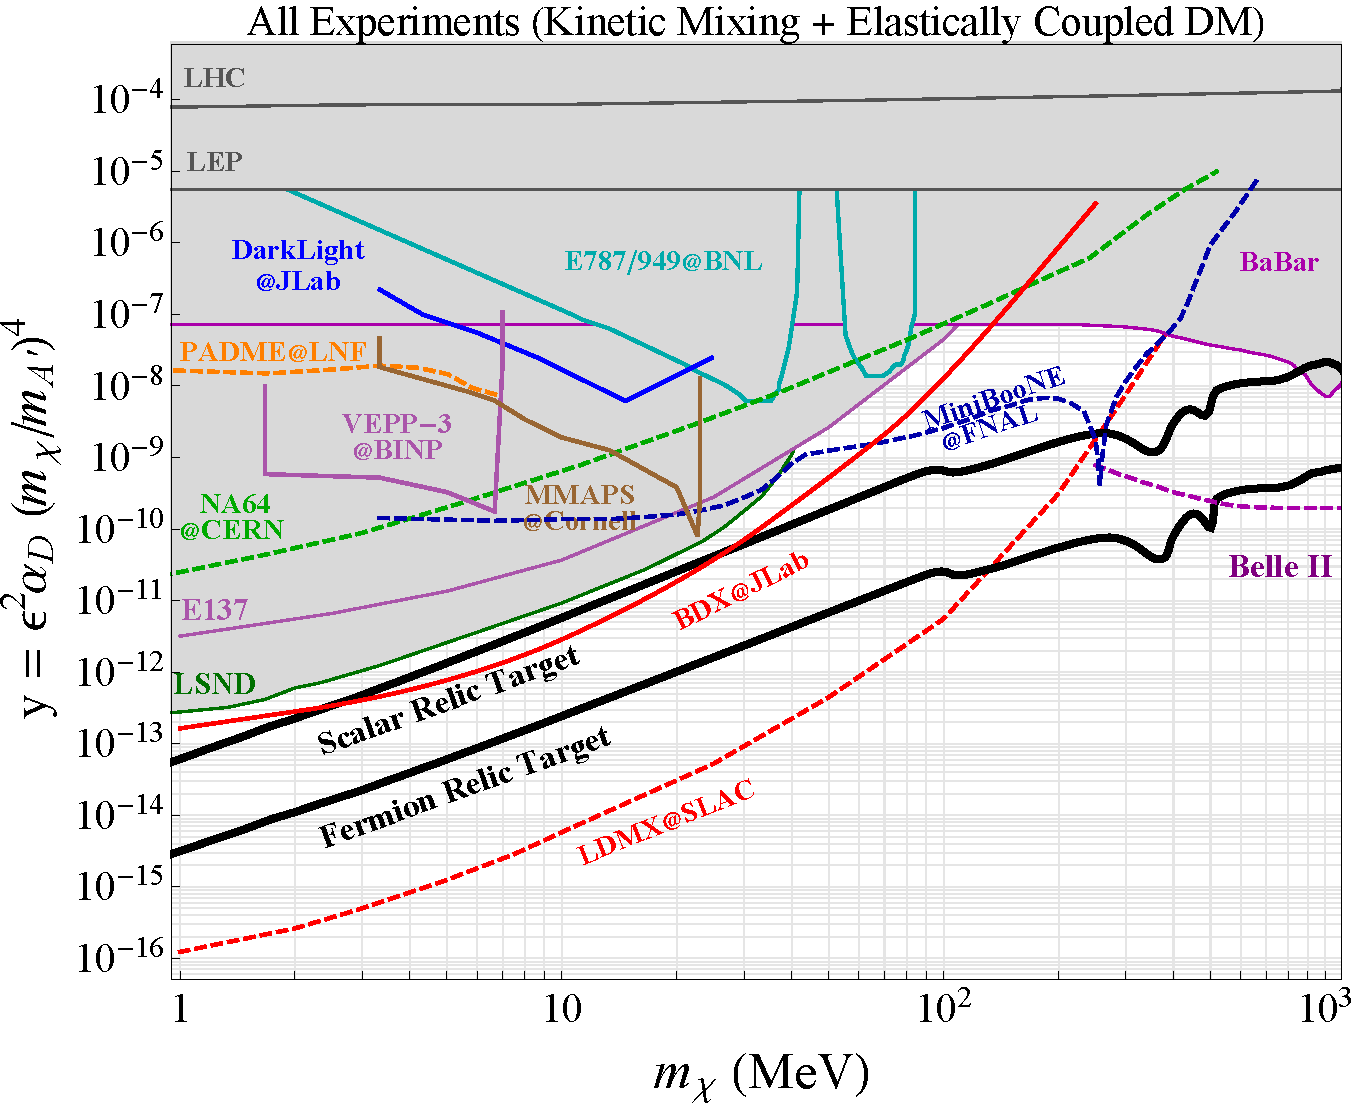
\includegraphics[width=11cm]{sections/goals/everything.pdf}
\caption{ The parameter space for LDM and future experimental projections in the $y$ vs. $m_\chi$ plane plotted against
 the thermal relic targets for scalar and fermion DM -- see text for a discussion. }
\label{fig:mainplot}
\end{figure}

2
Although LDM represent fully half of the viable thermal DM mass range, there has never been a dedicated search
for this class of models. Most constraints that apply to the scenarios considered here are reinterpretations (by theorists)
of experimental results collected for other purposes and fall into the following categories:

\begin{itemize}

\item {\bf CMB Power Spectrum:} LDM can annihilate to SM particles during the time of recombination and ionize the newly 
formed hydrogen, thereby modifying the CMB power spectrum in conflict with observations from PLANCK \cite{dodge}. 
If this annihilation is $s$-wave and the DM is particle symmetric, the CMB rules out  LDM below $\sim $10 GeV. However
if the annihilation is $p$-wave (easily achieved for a scalar DM candidate coupled to a dark photon mediator) or 
if the DM population is different at the time of CMB (e.g. asymmetric or Majorana inelastic, see \cite{Izaguirre:2015yja} for a discussion)  
 
\item {\bf Colliders:} Although high energy colliders (LHC, Tevatron, LEP) generally have poor sensitivity to LDM, high intensity B-factories 
can perform analogous searches for $e^+e^- \to \gamma A^\prime$ production and set impressive constraints in the 100 MeV - few GeV 
mass range. 

\item {\bf Beam Dumps: } The LSND proton beam dump experiment  \cite{deNiverville:2011it} is sensitive to LDM production and scattering
in their measurement of the electron-neutrino neutral current cross section. At LSND, DM can be produced in pion decays $\pi^0 \to \gamma A^\prime \to \gamma \chi \chi$
and subsequently scatter in a downstream detector.  The E137 electron beam dump experiment  to search for axion like particles is also sensitive to 
similar processes in which DM is relativistically  produced through the kinetic mixing interaction in the beam dump, passes through a downstream 
 detector and deposits electromagnetic energy by scattering off detector targets  \cite{Batell:2014mga}. 

\item{\bf Rare Kaon Decays}: LDM can also be produced in rare Kaon decays $K^+ \to \pi^+ A^\prime \to \pi^+ \chi \chi$ which 
can contribute to the signal region of E787/E949  \cite{Adler:1997am,Artamonov:2008qb} which measured the $K^+ \to \pi^+ \bar \nu \nu$ branching ratio. 

\item{\bf Electron Direct Detection}: The results of XENON10 S2-only study of electron recoil signals can be used to 
constrain LDM that scatters elastically off detector electrons \cite{Essig:2012yx}. Although the backgrounds for this sample are not well understood,
a conservative extraction of the DM scattering limit can be used to constrain this parameter space. This bound is competitive with 
E137 and E787/E949 in Fig. \ref{fig:main plot}, but is slightly covered by those constraints for the benchmarks presented, so it is not shown.

\end{itemize}

These constraints are collected in on the $y$ vs $m_\chi$ parameter space depicted in Fig. \ref{fig:mainplot}  alongside projections
for Belle II \cite{Essig:2013vha}, BDX \cite{Izaguirre:2013uxa,Battaglieri:2016ggd}, MiniBooNE \cite{Dharmapalan:2012xp}, NA64 \cite{Gninenko:2016kpg}, VEPP-3 \cite{Wojtsekhowski:2012zq}, and MMAPS \cite{cornell}.
Also shown are the thermal targets for fermion and scalar LDM candidates, which are invariant in this parameter space regardless
of what assumptions about $\epsilon, \alpha_D$, and $m_\chi/m_{A^\prime}$ we choose. However, the other constraints on this 
parameter space are not necessarily invariant in this way (e.g. collider production only depends on $\epsilon$), so the 
shaded regions in Fig. \ref{fig:mainplot} represent the most conservative versions of these constraints for which
 these parameters are chosen to reveal all the remaining gaps in the parameter space consistent with the assumption of 
 direct annihilation. 
 
 This plot illustrates the large, orders of magnitude gaps in coverage between existing (and projected) constraints
 and the thermal relic contours for LDM. In order to decisively cover thermal LDM in the direct annihilation regime, a dedicated effort will
 be required. To this end, we also show the projections for LDMX@SLAC, which is the only proposed effort to probe the thermal
 target for both scalars and fermions down to the MeV range. 

\subsection{Nuclear Physics Measurements}

Work in progress...



%%%%%%%%%%%%%%%%%%%%%%%%
%   Detector Concept   %
%%%%%%%%%%%%%%%%%%%%%%%%
\clearpage
\section{Detector Concept}

%%%%%%%%%%%%%%%%
%   Overview   %
%%%%%%%%%%%%%%%%

Basic Considerations and Overview
\begin{itemize}
    \item Signal characteristics
    \item Possible backgrounds 
    \item Achieving high luminosity 
    \item Explain why we want a tagger tracker, moderate 0.1 X0 target, recoil 
          tracker, high granularity calorimeter, hadronic veto
    \item Summarize the overall layout of the experiment 
\end{itemize}




%%%%%%%%%%%%%%%
%  Beamline   %
%%%%%%%%%%%%%%%

\subsection{Beamline, Magnet, and Vacuum Layout}


%%%%%%%%%%%%%%%%%%%%%
%  Tagger Tracker   %
%%%%%%%%%%%%%%%%%%%%%

\subsection{Tagging Tracker (Editors: Tim Nelson, Omar Moreno)}


%%%%%%%%%%%%%%
%   Target   %
%%%%%%%%%%%%%%

\subsection{Target (Editors: Tim Nelson, Omar Moreno)}


%%%%%%%%%%%%%%%%%%%%%
%  Recoil Tracker   %
%%%%%%%%%%%%%%%%%%%%%

\subsection{Recoil Tracker (Editors: Tim Nelson, Omar Moreno)}

The recoil tracker is designed to identify low-momentum (50 MeV - 1.2 GeV) recoils and precisely determine their momentum, direction and impact position at the target.  In addition, it must work together with the calorimeters to correctly distinguish low-momentum signal recoils from scattered beam electrons and multi-particle backgrounds. The key elements of the design are determined by this goal.  First, the recoil tracker is placed at the end of the magnet in the beginning of the fringe field to optimize tracking for particles up to two orders of magnitude softer than the beam energy electrons measured by the tagging tracker.  Second, the recoil tracker is short and wide for good acceptance in angle and momentum and to minimize the distance from the target to the calorimeters to improve their angular coverage. Finally, the recoil tracker provides 3-d tracking near the target for both direction and impact parameter resolution but emphasizes low mass density over the longest possible lever arm further downstream to deliver the best possible momentum resolution.  This design delivers good momentum resolution for both multiple-scattering limited low-momentum tracks and beam energy electrons that are nearly straight in the fringe field.

The layout of the recoil tracker is summarized in Table XXX and consists of four stereo layers immediately downstream of the target and two axial layers at larger intervals in front the the ECal.  The stereo layers are double-sided modules of silicon microstrips arranged at 15 mm intervals downstream of the target, with the first module centered at z=+7.5 mm.  These modules are laterally centered on the target and the center of the vacuum chamber and are identical to the modules of tagger tracker that are mounted upstream on the same support plate.  

The thinner axial-only layers, at z=+90 mm and z=+180 mm, are mounted on a separate support structure at the downstream end of the vacuum chamber as described in Section XXX and have a somewhat different module design.  Each module consists of a pair of sensors, glued end-to-end, with an APV25-based FR4 hybrid circuit board at each end of this structure to read out the two sensors. The sensors are standard p$^{+}$-in-n silicon microstrip sensors, but are somewhat shorter and wider than those used in the stereo modules and therefore require six APV25 chips to read out each sensor instead of five. The modules are supported at both ends by screw attachment of the hybrids to castellated support blocks attached to the cooled support structure. A vacuum compatible thermal compound is used to ensure good thermal conductivity between the hybrid and the support structure.

%%%%%%%%%%%%
%   Ecal   %
%%%%%%%%%%%%

\subsection{Forward Electromagnetic Calorimeter}


%%%%%%%%%%%%
%   Hcal   %
%%%%%%%%%%%%

\subsection{Hadronic Veto System}


%%%%%%%%%%%%%%%%
%   Wide cal   %
%%%%%%%%%%%%%%%%

\subsection{Wide-Angle Calorimeter ??}


%%%%%%%%%%%%%%%
%   Trigger   %
%%%%%%%%%%%%%%%

\subsection{Trigger System (Editors: Jeremy Mans, Nhan Tran, Andrew Whitbeck)}

The LDMX trigger system is designed to reduce the typical beam
particle arrival rate of $\approx 40$~MHz to a rate of \draft{O(1~kHz)} for
storage and analysis.  The selection is performed by a combination of
dedicated hardware and software running on general-purpose computers.

The first stage trigger is implemented in hardware and allows the
selection of both candidate events for dark matter production and
important samples for calibration and detector performance monitoring.
The overall trigger management is provided by a trigger manager board,
which receives inputs from the various triggering subsystems including
the silicon calorimeter and the scintillator calorimeter.  The latency
requirements on the trigger calculation latency are set \draft{by the tracker
  readout ASIC to 2us}.

The primary physics trigger is based on the silicon calorimeter and is
designed to select events with energy deposition significantly lower
than the full beam energy.  The silicon calorimeter ASIC calculates
the total energy in 2x2 fundamental cells for every 40~MHz
pseudo-bucket.  The energy information is transferred by digital data
link to the peripherary of the calorimeter, where sums can be made
over larger regions and transferred by optical link to the trigger
electronics.  The total energy is then used to select the events.

The use of a calorimeter trigger requirement of energy below a
threshold also requires a beam-presence measurement to avoid very high
trigger rates during crossings where there is no beam electron
present.  The trigger fiber hodoscope is designed to serve this
purpose.  The hodoscope is constructed of an array of \draft{1~mm}-diameter
scintillating fibers, which are mounted immediately upstream of the
tungsten target. \draft{[more details on the mechanics, including orientation
of the fibers]}

\begin{figure}[t]
  \caption{Drawing of the trigger fiber hodoscope}
\end{figure}

The fibers from the hodoscope are brought to an optical vacuum
feedthrough and a clear fiber ribbon is connected on the outside of
feedthrough to carry the light signals to the readout electronics.
Based on studies by the LHCb collaboration\cite{lhcb:scintfiberrad},
scaled to the diameter of fibers in use for the hodoscope, we expect a
typical signal of \draft{[]} photons to be produced in the hodoscope by a beam
electron after a total absorbed radiation dose of \draft{XXX Gray}.
We expect to able to bring at least \draft{[50\%]} of these photons
to the readout SiPMs.

The same electronics design is used for readout of the hodoscope and
the scintillator calorimeter.  This readout is based on SiPMs and the
housing is designed to allow operation of the SiPMs at reduced
temperatures (below $5^\circ$C) to reduce the thermally-induced
single-photon noise.  The typical photodetector efficiency of these
SiPMs is \draft{[30\%]}\cite{cms:sipm_performance}, providing a typical signal
of \draft{[]} PEs in the electronics.  The readout electronics will
continuously digitize the SiPM signal, providing an integrated charge
as well as time-of-arrival measurement for the pulse with an LSB of
500~ps.  Both amplitude and timing information can be provided to the
trigger, allowing the correction of the calorimeter amplitude for
timewalk effects already at trigger level.




%%%%%%%%%%%
%   DAQ   %
%%%%%%%%%%%

\subsection{DAQ}




%%%%%%%%%%%%%%%%%%%%%%%%%%%%%%%%%%%%%%%
%   Physics and Detector Simulation   %
%%%%%%%%%%%%%%%%%%%%%%%%%%%%%%%%%%%%%%%
\clearpage
\section{Physics and Detector Simulation}


%\subsection{Simulations Overview (Editors: Natalia Toro, Jeremy McCormick)}
\subsection*{\draft{Simulations Overview (Editors: Natalia Toro, Jeremy McCormick)}}
I don't think this should be a numbered section, but am keeping
This section describes the methods used to simulate signal and background physics reactions and the responses of various detectors to these reactions.  
For historical reasons, two separate simulation frameworks have been used: the ``tracker simulation'' implemented in SLIC comprises a full simulation of the tagger tracker and recoil tracker, with ECAL material included but not its detector response.  Likewise, the ``calorimeter simulation'' implemented directly in Geant4 comprises a full simulation of the ECAL and HCAL, with recoil tracker material included upstream. In both cases, the target material and magnetic field map are also included. \draft{Please check for accuracy} These two simulations are described in more detail in \S\ref{ssec:sim-tracker}--\ref{ssec:hcal}.

While the primary simulation engine is Geant4 \cite{g4}, the signal reaction (Dark Matter pair production) is modelled using an external generator based on MadGraph4 \cite{MG4}.  This generator, its validation, and the interface with Geant4 are described in \S\ref{ssec:signal}.  All background processes are modelled directly in Geant4, with modifications and biasing for photonuclear processes as discussed in \S\ref{ssec:photonuclear}.


\subsection{Simulation of the Tagger and Recoil Trackers (Editors: Omar Moreno, Jeremy McCormick)}

The simulation of the passage of both charged and neutral particles through 
the tagger and recoil trackers as well as the target uses a software 
package, the Simulator for the Linear Collider (SLIC)~\cite{}, based on the
GEANT4 toolkit. It creates realistic charge depositions in the silicon layers,
simulates the APV25 readout chip amplifier chain, creates clusters and performs
track finding and reconstruction.
The simulation is used to understand the track reconstruction efficiencies,
purity and to evaluate the momentum and vertex resolutions. A rendering of
the tagger and recoil tracker as used in the simulation is shown on 
Figure~\ref{}.
\begin{figure}
\end{figure}

%The performance studies assumed that the 
%tagger (recoil) tracker is within a uniform dipole field of strength -1.5 T 
%(-.75 T), while all acceptance studies use the full field map.

\subsubsection{Hit Reconstruction}

The charge depositions created by a particle in the silicon planes are used to
form strip hits. The signal present on each of the strips is used to simulate 
the APV25 pulse shape which is then sampled into a readout pipeline in intervals
of 24 ns. The six samples emerging from each channel are fit using a 3-pole 
function in order to extract the rise and fall time, the amplitude and time of 
the hit.
%\begin{equation}
%    f(t) = A\frac{\tau_1^2}{(\tau_1 - \tau_2)^3}\left( e^{-\frac{t-t_{0}}{\tau_1}}
%        - \sum_{k=0}^2 \left(\frac{\tau_1 - \tau_2}{\tau_1\tau_2}(t-t_{0})\right)^k
%        \frac{e^{-\frac{t-t_{0}}{\tau_2}}}{k!} \right)
%\end{equation}
%where $\tau_1$ and $\tau_2$ represent the fall and rise time of the shaper 
%signal respectively.  The amplitude, $A$, and the time of the hit, $t_0$, are then
%determined from the fit.

Hits on neighboring strips are clustered using a nearest neighbor
algorithm.
%as follows: 
%\begin{itemize}
%    \item A list of seeds is created from all raw hits that have an amplitude, $S$,
%          $> 4\times \sigma_{\text{Noise}}$
%  \item Recursively add neighboring strips that have $S> 3 \times \sigma_{\text{Noise}}$
%          until a strip with $S < 3\times \sigma_{\text{Noise}}$ is found.
%      \item Require that neighboring hits have a $t_{0}$ that is within 8 ns of the seed hit.
%    \item Repeat the first two steps until seed strips are no longer found.
%\item Require that a cluster has an amplitude $> 4 \times \sigma_{\text{Noise}}$.
%\end{itemize}
After hits on a sensor have been
clustered, the cluster time is computed as the amplitude-weighted average
of the $t_0$ times from the hits that compose it. All clusters in adjacent pairs
of layers are combined to create 3D hits used by the track finding and fitting
algorithm.

\subsubsection{Track Reconstruction}

The track finding and fitting algorithm proceeds in steps following a specific 
``tracking strategy''.  The strategies outline which layers are used, the 
minimum number of hits required to form a track and kinematic constraints.  
The algorithm proceeds as follows:
\begin{itemize}
    \item All possible combinations of hits are formed from the seed layers and
          and a helix fit is performed.  Only those seeds which satisfy a 
          $\chi^2$ requirement are kept. 
    \item Once all seeds have been found, hits from a specified ``confirm'' 
          layer are added to the seeds and a helix fit is performed once again.
          Those fits which do satisfy a $\chi^2$ cut are eliminated.
    \item Finally, tracks are ``extended'' by hits from the rest of the layers.
          After the addition of a hit, a helix fit is performed.  If the track
          fails the $\chi^2$ constraint, the hit is discarded.  This procedure
          is repeated until all hits in a layer have been added to all seeds, 
          however, it is possible for all hits in a layer to be discarded.
    \item All track candidates are merged in order to form a set of unique 
          tracks.  Tracks are allowed to share at most one hit.  If a pair of
          tracks shares more than a single hit, the track with the best $\chi^2$ 
          is chosen. 
\end{itemize}



\subsection{Simulation of the Forward Electromagnetic Calorimeter (Editors: Owen Colegrove, Joe Incandela)}


\subsubsection{Digitiztaion of the Hadronic Veto System (Editors: Nhan Tran, Andrew Whitbeck)}
\label{sec:hcaldig}

After full {\tt GEANT4} simulation, we simulate the digitization of the particle-level interactions in our detector to 
understand how well we can reconstruct events in the hadronic calorimeter.  Given the particle-level energy 
deposition per layer, we can convert that into the an expected number of photo-electrons (PEs).   
{\tt GEANT4} simulations with 4 GeV incident muons are used to estimate the expected detector response to minimum ionizing particles (MIPs).  Fig.~\ref{fig:hcalMIP} shows the distribution of energy deposited in a given layer of scintillator; on
average, each MIP deposits 1.4 MeV of energy in a given layer.   For each MIP, we assume that 20 PEs are detected
on average.

The digitization parameters used in these studies are based on CMS test beam measurments~\cite{}, where 
the mean MIP response was 13.5 PEs for a comparable HCal geometry.  This MIP response has been scaled up to
account for the differences in scintillator thinkness, assuming that the light collection efficiency will remain constant.

The sum of SiPM and electronics noise is expected to be 2 PEs.  Although noise is not explicitly simulated, only layers
that have a minimum of 8 PEs are considered in further studies.   Thus, noise affects are expected to be negligible.  



\begin{figure}[hbtp]
\begin{center}
    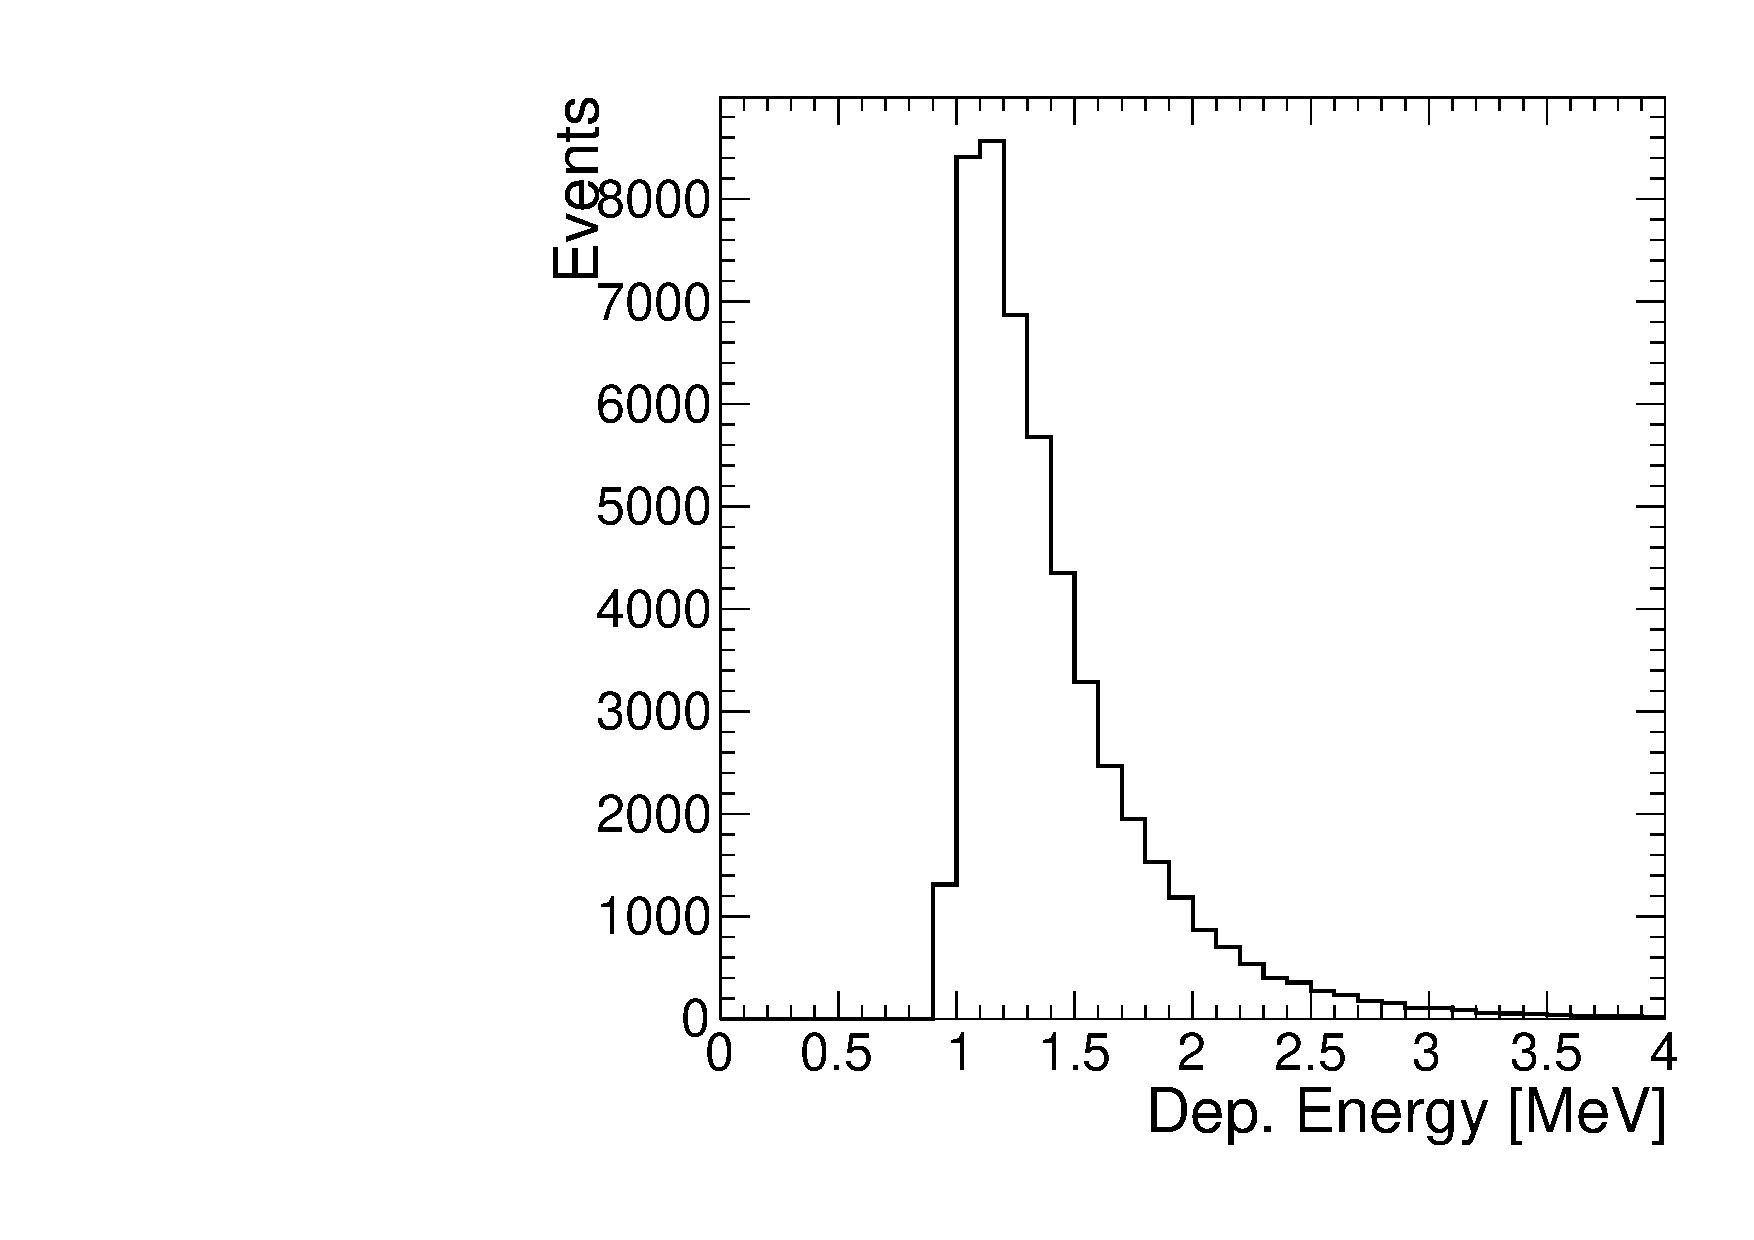
\includegraphics[width=0.5\textwidth]{images/hcal/MIPresponse0degreesOnly.pdf}
    \caption{Distribution of energies deposited in scintillator from muon to characterize MIP behavior in plastic scintillator}
 \label{fig:hcalMIP}
 \end{center}
\end{figure}



\subsection{External Physics Generator for Signal Reaction (Dark Matter Production) (Editor: Natalia Toro)}
While background processes are modelled entirely in the Geant4 framework, the new physics of Dark Matter production is modelled using an external event generator based on MadGraph/MadEvent4 \cite{MG4}.  Here we describe this generator, its validation, and the interface with Geant4.

MadGraph is an automated tool for calculating the tree-level amplitudes for arbitrary physics processes, which allows users to define Feynman rules for new physics models; MadEvent is a Monte Carlo event generator based on MadGraph.  MadGraph/MadEvent4 (MG/ME) was designed for the study of high-energy collider reactions, but minor modifications to the code (introducing non-zero masses for incident particles and for the electron, and an electromagnetic form factor as described in \cite{Tsai} for the nucleus) allow for its application to fixed-target processes.  These modifications and a new-physics model that introduces a dark photon with arbitrary mass and kinetic mixing $\epsilon$ with the photon has been used for  the APEX test run \cite{APEXtest} and HPS experiment \cite{HPStest}.  For LDMX, we have added light dark matter particles (either fermions or scalars) that couple to the dark photon with an arbitrary interaction strength $g_D$.  This allows us to simulate the signal process of DM particle pair-production via either decay of an on-shell $A'$ or off-shell $A'$ exchange.   This report focuses on the on-shell production process, though the kinematics of the two are very similar.  

\draft{Do we want to say something explicit about the form factors?}

Within MG/ME, we generate events for the DM production process $e^- W \rightarrow e^- W \,(A^\prime \rightarrow \chi \bar\chi)$ where $\chi$ represents the dark matter particle and $\bar\chi$ its antiparticle. Events are generated assuming a 4 GeV incident electron and Tungsten nucleus at rest as the initial state.  MG/ME computes a Monte Carlo approximation of the inclusive cross-section for this process, and generates a sample of unweighted events in the Les Houches Event (LHE) format \cite{LHE}.  The inclusive cross-section computed by MadGraph is stable within $1\%$ and is consistent within $\sim 30\%$ with independent calculation of the cross-section in the Weizsacker-Williams (WW) approximation from \cite{Andreas09}.  The deviations from the WW inclusive cross-section are largest at high and low masses, and compatible with the size of errors expected in the WW approximation.

\draft{[IS THSI RIGHT?] To seed Geant4 events from the MG/ME output, we read the four-momentum of the recoiling electron \draft{and Tungsten nucleus??} from the LHE file and use these to populate an STDHEP event.  The electron and nucleus are assumed to originate from a common vertex, uniformly distributed over the thickness of the target and over a transverse region spanning \bf{CHECK!} $\pm 1 \cm$ in the $x$ direction and $\pm 2 \cm$ in the $y$ direction about the nominal center of the target.}




\subsection{Photonuclear Model and Biasing (Editors: Natalia Toro, Omar Moreno)}



%%%%%%%%%%%%%%%%%%%%%%%%%%%
%   Performance Studies   %
%%%%%%%%%%%%%%%%%%%%%%%%%%%
\clearpage
\section{Performance Studies}

Baseline luminosity:  We want to handle $4\times 10^{14}$ electrons on target (EOT) with incoming energy of $4$ GeV. 

\subsection{Signal Characteristics}

Please note that we need to optimize the energy selection used below. Starting definition: 

Tracking: 

- one incoming beam electron with $E_{beam}$ close to $4$ GeV and a well measured trajectory. 
 
- quality cuts (as needed) to reduce any dangerous brem (or photo-nuclear) reactions in the tagger tracker material
 
- one recoiling electron with $E\lesssim 1.2$ GeV that points back to the incoming beam electron track. 

- an activity cut in the recoil tracker to reject photo-nuclear reactions in the target

- an inferred ``missing momentum'' trajectory and magnitude 

Calorimetry: 

- one soft recoil shower with $E\lesssim 1.2$ GeV that is consistent with recoil tracker trajectory

- an activity cut in the ``missing momentum'' region for the ECal

- an explicit veto on energetic (energy range needs to be specified) hadrons in both the ECal and hadron veto system 

\subsection{Tagging Tracker Performance}

Needs to be spelled out in more detail...

- acceptance

- efficiency 

- purity (THIS ONE IS CRITICAL)

\subsection{Recoil Tracker Performance}

Needs to be spelled out in more detail...

- acceptance

- efficiency 

- what kind of activity cuts do we want to apply?  Background rejection power?  Signal efficiency? 


\subsection{Forward Electromagnetic Calorimeter}

Owen and Joe will discuss this at the July 8 meeting. But Philip's notes include: 

- Hermiticity:  make sure to include a study of cracks or dead material in the detector simulation. Do we need to worry about this? Why? 

Large scale ``top down'' monte carlo study to demonstrate baseline performance of ECal and to justify more detailed study of specific reactions that dominate the tail of low energy deposition events. We need to quantify everything I'm about the say more carefully. Starting from $4\times 10^{14}$ EOT, the baseline tracker selections bring the event sample down to $\sim 4 \times 10^{12}$. So we're dealing with $\sim 4 \times 10^{12}$ events with a soft recoiling electron and a hard, $\sim 3$ GeV, photon. ECal events that are hadron rich occur about $\sim10^{-3}$ of the time. So now we're down to $\sim 4\times 10^{9}$ hadron rich events in the ECal. 

- most importantly, we want to understand what dominates the low energy deposition events

- we want to characterize the hadron rich events (because we know they are a potential issue)

- explain veto strategy

- at what point is the energy deposition so low that it's not possible to veto effectively? what are these events types? 

Specific ``bottom up'' studies of photo-nuclear reactions:  We know that certain event types could pose a challenge, so let's study them. The numbers shown below are with very loose kinematic selections, so they are upper bounds. They are also for $9$ GeV photons, so Philip and Natalia will need to correct them. This is a good starting point for study however: 

- $\gamma N \rightarrow (\rho,\omega,\phi)N\rightarrow \pi^+\pi^- N$ ($\lesssim 10^8$ of this event type). 

- $\gamma N \rightarrow  \mu^+\mu^- N$ ($\lesssim 2 \times 10^7$ of this event type). 

- $\gamma p \rightarrow \pi^+ n$ ($\lesssim 4\times 10^5$ with $\sim 4\times 10^3$ of these having a backscattered $\pi^+$). 

- $\gamma n \rightarrow n \bar{n} n$ ($\lesssim 4\times 10^5$ of this type). 

- $\gamma (p,n) \rightarrow K_L K_L + X$ (expect this at the $\sim 10^3$ level, but we need to check this!)

The current plan is to use a particle gun and weight the depth of origination and angle/energy distribution using data. Let Philip and Natalia know when you're ready to do this. 
{\it We need to be especially careful to include the regions of phase space where the MIPs are soft or wide/back scattering by recoiling off the nucleons or atoms. This needs a dedicated study, starting with the physics simulations group, P,N,E,G}. 


\subsection{Hadronic Veto System}

A good starting point would be to focus on the event types that the ECal will certainly have a tough time with. These are the few-body photo-nuclear reactions for sure. So it might make sense to start with the ``bottom up'' study outlined above. 

\subsection{Trigger}

We need to spell out our trigger streams. 

Signal stream: 

- a single cluster with energy below $\sim ??$ GeV. 

- coincident with a signal from the fast-or layer in the tracker

- rate? 

What other streams do we need to measure performance? 


%%%%%%%%%%%%%%
%   Budget   %
%%%%%%%%%%%%%%
\clearpage
\section{Budget and Schedule}

\subsection{DASEL}

\subsection{Tracking}

\subsection{Forward ECal}

\subsection{Hadronic Veto}

\subsection{Trigger}

\subsection{DAQ}

\subsection{Operations}



%%%%%%%%%%%%%%%%%%%%
%   Bibliography   %
%%%%%%%%%%%%%%%%%%%%
\bibliographystyle{JHEP}
\bibliography{bibliography}

\end{document}

